\chapter{Architektura aplikace}\label{sec:ApplicationTechnology}

\section{Zvolený návrh}

Aplikace je členěná na 3 základní knihovny, což je zřejmé na obrázku \ref{fig:ARCH}.
Každá část má vlastní účel a jsou navzájem izolovány.
První z těchto knihoven je \textbf{regexer}, ta slouží pro zpracovávání a vyhodnocování regulárních výrazů.
Jako jediná z těchto knihoven může existovat plně nezávisle na ostatních knihovnách, jelikož neobsahuje závislost na žádné z dalších knihoven.
Druhou knihovnou je \textbf{vizualizační}, která slouží pro samotné zobrazení zpracovávaných regulárních výrazů.
Jedná se o komponentu, která může být spuštěná mimo rozšíření VSCode, například ve webovém prostředí.
Tato knihovna obsahuje závislost na Regexer, ale na VSCode extension není přímá závislost, jelikož pokud není nalezená funkce pro zasílání zpráv, tak je v rámci vizualizace ignorována.
Poslední částí je samotné \textbf{rozšíření}, které se stará o komunikaci s API VSCode a o řízení všeho co se týká rozšíření.
Tato část aplikace implementuje vizualizační knihovnu v podobě webview (webové zobrazení).

Na obrázku \ref{fig:ARCH} je viditelná závislost mezi knihovnami. 
Rovněž je patrná základní struktura těchto knihoven a jejich závislosti mezi sebou.
Avšak jsou zakresleny jen ty komponenty, které můžeme považovat za nejdůležitější. 
Je dobré zdůraznit asynchrony komunikaci, kterou poskytuje knihovna regexer (vyhodnocující regexy).
Tuto komunikaci lze vidět mezi komponentou Regexer a RegexVisualizer s tím, že Regexer využívá vedlejší vlákno mimo hlavní. 
Knihovna pro vlákna threads.js je popsána v sekci \ref{sec:USEDtech}.

% TODO: zkusit zvětšit
\begin{figure}[!h]
	\centering
	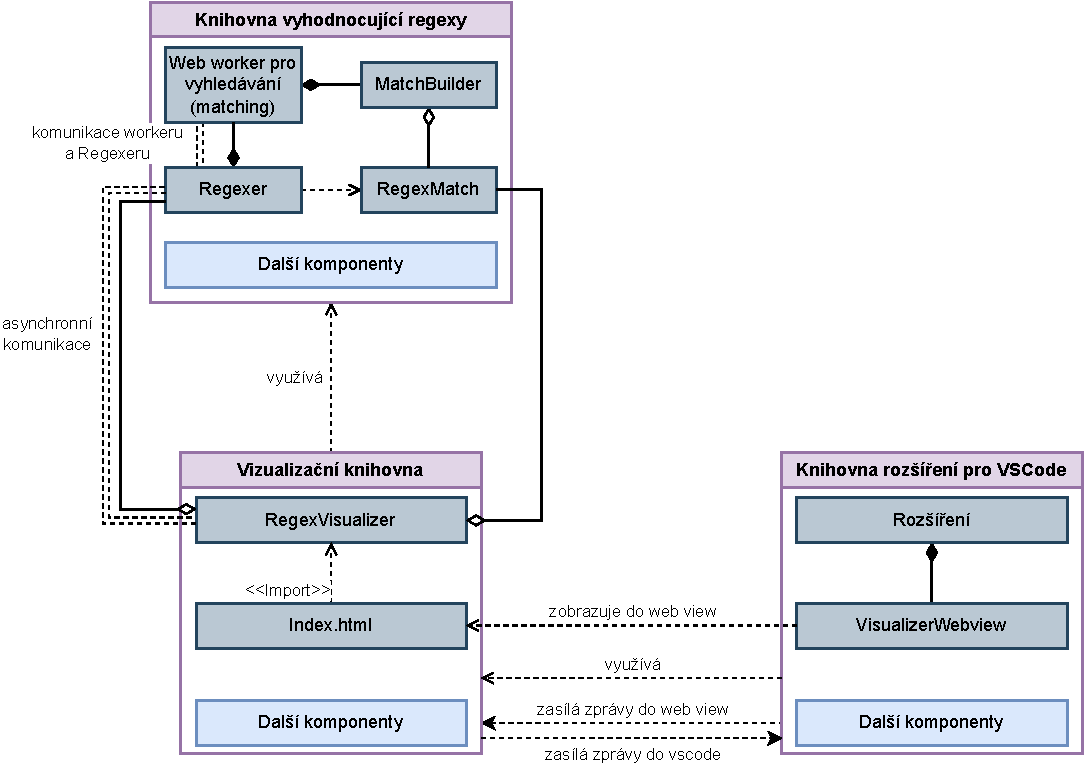
\includegraphics[width=.9\textwidth]{Figures/BP-Arch.pdf}
	\caption{Struktura knihoven aplikace}
	\label{fig:ARCH}
\end{figure}

\newpage

\section{Použité technologie}\label{sec:USEDtech}
Tato aplikace je integrovaná do vývojového prostředí \textbf{visual studio code}, 
zkráceně \textit{VSCode}. Jádro aplikace je psáno v programovacím jazyce \textbf{TypeScript}, zkráceně \textit{TS} verze 5.3, který je nadstavbou
pro jazyk \textbf{JavaScript}, zkráceně \textit{JS}. TypeScript má jako hlavní nadstavbu, možnost využívání a přiřazování datových typů.
Také platí, že kód napsaný v JS je správný pro TS, ale to neplatí naopak.
Psaní větší aplikace je tak často vhodnější v TS, 
kvůli svým typovým kontrolám, čímž se jako programátor mohu vyvarovat potencionálním chybám při běhu programu.
Také vývojové prostředí VSCode, zpřístupňuje API pouze pro JavaScript nebo TypeScript.
Sice by bylo možné mít část aplikace napsané v jiném jazyce, to by ale mělo své komplikace při vývoji.

Pro parsování jsem se rozhodl použít bezkontextovou gramatiku \textbf{Peggy}\cite{Peggy, Peggyjs}, pro jazyk JavaScript.
Ta umožňuje poměrně snadného zpracování textové podoby regulárních výrazů, do podoby nějaké struktury.
Tato výsledná struktura může být v podstatě jakákoliv.

Všechny části aplikace, jsou zpravovány balíčkovým manažerem \textbf{NPM} (Node Package Manager).
Také využívají některých balíčků, které jsou dostupné pro npm. 
Část aplikace je pak postavená na technologii \textbf{NodeJS}.
Jedná se o JavaScript runtime (běh programu). 
Například runtime VSCode rozšíření je NodeJS, oproti tomu samotné webview běží na klasickém webovém runtime, které je typické pro webové prohlížeče.

Vizualizační část aplikace pak využívá základní \textbf{HTML} struktury.  
HTML je základem pro webové stránky a definuje jejich strukturu pomocí značek.
Pro následnou změnu vzhledu (styl), jsem využil technologie \textbf{LESS}\footnote{https://lesscss.org/}, což je rozšíření standardního \textbf{CSS}.
Avšak LESS musí být transpilovaný\footnote{Typ překladu z jednoho jazyka na jazyk jiný} do CSS, jelikož webová stránka ho nezná. 
LESS umožňuje, například vnořování stylů nebo tvorbu vlastních proměnných.
Pro logickou část vizualizační knihovny je také využit TypeScript.

Pro výsledný přeložený kód, je použit balící nástroj \textbf{Webpack}\footnote{https://webpack.js.org/}.
Ten mi umožňuje, všechny části aplikace poměrně efektivně zabalit, do malého počtu souborů. 
Tento nástroj se pak hodí, pro menší výslednou aplikaci a hlavně pro seskupení všech závislostí.
Mohu mít i větší kontrolu nad výsledným kódem.
Například lze udávat, kdy se mají soubory dělit, jak se mají zpracovávat přílohy, jako jsou obrázky atd.
Pro optimalizaci a úpravu kódu, se zde využívá takzvaných \textit{loaderů} a \textit{pluginů}, 
které dokážou v určité části překladu zasáhnout a popřípadě změnit určitou část kódu.
Ve výsledku se jedná o velice silný nástroj, který dává programátorovi větší kontrolu nad výsledným přeloženým kódem aplikace.

Jelikož jsem chtěl mít větší jistotu, nad správností aplikace, je v algoritmické části aplikace využito technologie pro tvorbu testů. 
Tato knihovna se nazývá \textbf{Jest}\footnote{https://jestjs.io/}.
Avšak tato knihovna slouží převážně pro testování JavaScriptových kódů, proto jsem k ní využil balíčku \textbf{ts-jest}\footnote{https://www.npmjs.com/package/ts-jest}, pro TypeScript.
To mi pak umožňuje psát testy, které mohou využít typů.

Jednou z posledních knihoven, kterou jsem použil, je \textbf{Threads.js}\footnote{https://threads.js.org/}. 
Jelikož existují různé runtime JavaScriptu, tak neexistuje jednotný standard pro implementaci vláken (threads).
Browser má tzv. \textit{web workery} a NodeJS má \textit{worker thready}, sice si jsou podobné, ale mají změny které znemožňují univerzálního použití.
Proto je v této aplikaci využito threads.js, které eliminuje tyto problémy.
Navíc dokáže nabídnout větší bezpečnost pro programátora, který píše kód v TS. 
Tato bezpečnost je docílená tím, že knihovna dokáže poskytnout z vlákna rozhraní, které může obsahovat i typy.

% TODO: popsat peggy syntax
\endinput